\documentclass[12pt]{article}

%===============================
%
%          📦 Paquetes
%
%===============================

\usepackage[a4paper, top=3cm, bottom=4cm, left=2.5cm, right=2.5cm]{geometry}
\usepackage[spanish]{babel}
\usepackage[utf8]{inputenc}
\usepackage{amsmath}
\usepackage{multicol}
\usepackage{graphicx}
\usepackage{hyperref}
\usepackage{booktabs}
\usepackage{pgfplots}
\usepackage{makecell}
\pgfplotsset{compat=1.18}

\title{
  \vspace{2cm}
  \pagenumbering{gobble}
  
\includegraphics[width=5cm]{../assets/logo-utp.png} \\
  \vspace{1cm}
  \textbf{Universidad Tecnológica del Perú} \\
  \vspace{2cm}
  \textbf{Investigación Operativa} \\
  \vspace{1cm}
  \large \textbf{S10 - Ejercicios}
}
\author{
  \textbf{Torres Vara, Mateo Nicolas} - \texttt{U24308542} \\
  \texttt{Sección 36373}
}



\begin{document}
\maketitle
\begin{center}

  Docente: Alberto Andre Reyna Alcantara

\end{center}

%======================================
%
%          📚 Inicio del documento
%
%======================================

\newpage
\pagenumbering{arabic}
\section*{Ejercicio 1}
\noindent Se tiene 3 plantas que abastecen a 2 distribuidores que envían los productos a 3
tiendas. A continuación, se presentan los datos del caso:

\begin{center}
\begin{tabular}{|c|c|c|c|}
\hline
& \multicolumn{3}{c|}{Plantas} \\ 
\hline
& A & B & C \\ 
\hline
Costo de producción (\$/unidad) & 10 & 12 & 9 \\
\hline
Capacidad de producción (unidades) & 1000 & 1200 & 800 \\
\hline
\end{tabular}
\end{center}

\vspace{1cm}

\begin{center}
\begin{tabular}{|c|c|c|}
  \hline
  & \multicolumn{2}{c|}{\makecell{Costo de transporte desde \\  las plantas a los \\ distribuidores (\$/unidad)}} \\
  \hline
  & Distribuidor 1 & Distribuidor 2 \\
  \hline
  Planta A & 2 & 1 \\
  \hline
  Planta B & 2 & 3 \\
  \hline
  Planta C & 2 & 2 \\
  \hline
\end{tabular}
\end{center}

\vspace{1cm}

\begin{center}
\begin{tabular}{|c|c|c|c|}
  \hline
  & Tienda 1 & Tienda 2 & Tienda 3 \\
  \hline
  Precio de Venta (\$/unidad) & 32 & 32 & 30 \\
  \hline
\end{tabular}
\end{center}

\vspace{1cm}

\noindent La capacidad de cada distribuidor es 2000 unidades. Además, el inventario inicial en el
distribuidor 1 es de 50 unidades, y en el distribuidor 2 es 100 unidades.

\begin{center}
\begin{tabular}{|c|c|c|c|c|c|c|}
  \hline
  & \multicolumn{6}{c|}{Demanda Máxima}\\
  \hline
  & Mes 1 & Mes 2 & Mes 3 & Mes 4 & Mes 5 & Mes 6 \\
  \hline
  Tienda 1 & 1200 & 1400 & 2000 & 1800 & 1600 & 1200 \\
  \hline
  Tienda 2 & 1100 & 1600 & 1400 & 1800 & 1200 & 1600 \\
  \hline
  Tienda 3 & 1400 & 1800 & 1500 & 1700 & 1300 & 1600 \\
  \hline
\end{tabular}
\end{center}

\vspace{1cm}

\noindent\textbf{Resolver:}
\begin{itemize}
  \item[1.] Formular el modelo correspondiente para maximizar la utilidad.
  \item[2.] Indique los inventarios mes a mes en cada distribuidor. 
\end{itemize}

\subsection*{Formulación del modelo lingo}
\begin{center}
  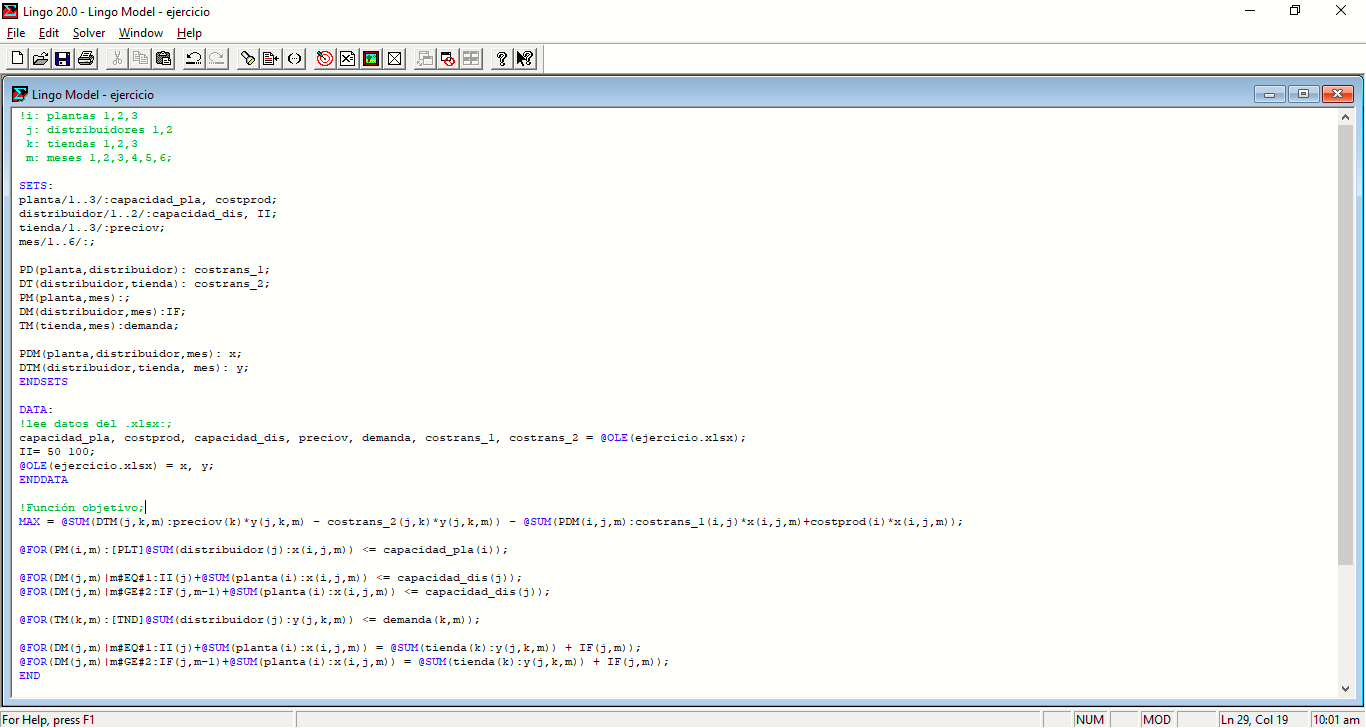
\includegraphics[width=\linewidth]{assets/modelo-lingo.PNG}
\end{center}

\vspace{3cm}

\subsection*{Resultados}
\noindent Referirse al excel para claridad de los resultados.
\begin{center}
  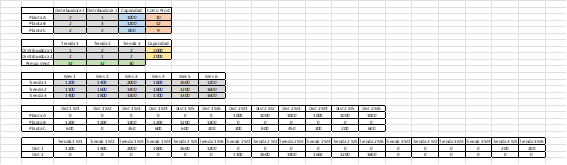
\includegraphics[width=\linewidth]{assets/resultados.png}
\end{center}

\subsection*{Inventarios mes a mes de cada distribuidor}
\begin{center}
\begin{tabular}{c c}
  % left cell: image
  \begin{minipage}[t]{0.4\linewidth}
    \vspace{0pt} % important: remove baseline offset
    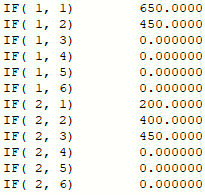
\includegraphics[width=\linewidth]{assets/inventarios.PNG}
  \end{minipage}
  &
  % right cell: table
  \begin{minipage}[t]{0.4\linewidth}
    \vspace{1pt}
    Los inventarios mes a mes en cada distribuidor son los siguientes: \\\\
    \vspace{0pt}
    \begin{tabular}{|l|c|c|}
      \hline
      & Distribuidor 1 & Distribuidor 2 \\
      \hline
      Mes 1 & 650 & 200 \\
      \hline
      Mes 2 & 450 & 400 \\
      \hline
      Mes 3 & 0 & 450 \\
      \hline
      Mes 4 & 0 & 0 \\
      \hline
      Mes 5 & 0 & 0 \\
      \hline
      Mes 6 & 0 & 0 \\
      \hline
    \end{tabular}
  \end{minipage}
\end{tabular}
\end{center}

\vspace{3cm}

\section*{Recursos y créditos}

\begin{itemize}
  \item \textbf{Código fuente:} \href{https://github.com/MateoTVara/UTP}{Repositorio GitHub - Investigación Operativa}
  \item \textbf{Carátula por:} \href{https://github.com/1nfinit0}{1nfinit0 en GitHub}
\end{itemize}

\end{document}